\PassOptionsToPackage{unicode=true}{hyperref} % options for packages loaded elsewhere
\PassOptionsToPackage{hyphens}{url}
%
\documentclass[ignorenonframetext,]{beamer}
\usepackage{pgfpages}
\setbeamertemplate{caption}[numbered]
\setbeamertemplate{caption label separator}{: }
\setbeamercolor{caption name}{fg=normal text.fg}
\beamertemplatenavigationsymbolsempty
% Prevent slide breaks in the middle of a paragraph:
\widowpenalties 1 10000
\raggedbottom
\setbeamertemplate{part page}{
\centering
\begin{beamercolorbox}[sep=16pt,center]{part title}
  \usebeamerfont{part title}\insertpart\par
\end{beamercolorbox}
}
\setbeamertemplate{section page}{
\centering
\begin{beamercolorbox}[sep=12pt,center]{part title}
  \usebeamerfont{section title}\insertsection\par
\end{beamercolorbox}
}
\setbeamertemplate{subsection page}{
\centering
\begin{beamercolorbox}[sep=8pt,center]{part title}
  \usebeamerfont{subsection title}\insertsubsection\par
\end{beamercolorbox}
}
\AtBeginPart{
  \frame{\partpage}
}
\AtBeginSection{
  \ifbibliography
  \else
    \frame{\sectionpage}
  \fi
}
\AtBeginSubsection{
  \frame{\subsectionpage}
}
\usepackage{lmodern}
\usepackage{amssymb,amsmath}
\usepackage{ifxetex,ifluatex}
\usepackage{fixltx2e} % provides \textsubscript
\ifnum 0\ifxetex 1\fi\ifluatex 1\fi=0 % if pdftex
  \usepackage[T1]{fontenc}
  \usepackage[utf8]{inputenc}
  \usepackage{textcomp} % provides euro and other symbols
\else % if luatex or xelatex
  \usepackage{unicode-math}
  \defaultfontfeatures{Ligatures=TeX,Scale=MatchLowercase}
\fi
% use upquote if available, for straight quotes in verbatim environments
\IfFileExists{upquote.sty}{\usepackage{upquote}}{}
% use microtype if available
\IfFileExists{microtype.sty}{%
\usepackage[]{microtype}
\UseMicrotypeSet[protrusion]{basicmath} % disable protrusion for tt fonts
}{}
\IfFileExists{parskip.sty}{%
\usepackage{parskip}
}{% else
\setlength{\parindent}{0pt}
\setlength{\parskip}{6pt plus 2pt minus 1pt}
}
\usepackage{hyperref}
\hypersetup{
            pdftitle={Tabla de contingencia},
            pdfauthor={Juan Ramon Lacalle},
            pdfborder={0 0 0},
            breaklinks=true}
\urlstyle{same}  % don't use monospace font for urls
\newif\ifbibliography
\usepackage{color}
\usepackage{fancyvrb}
\newcommand{\VerbBar}{|}
\newcommand{\VERB}{\Verb[commandchars=\\\{\}]}
\DefineVerbatimEnvironment{Highlighting}{Verbatim}{commandchars=\\\{\}}
% Add ',fontsize=\small' for more characters per line
\usepackage{framed}
\definecolor{shadecolor}{RGB}{248,248,248}
\newenvironment{Shaded}{\begin{snugshade}}{\end{snugshade}}
\newcommand{\AlertTok}[1]{\textcolor[rgb]{0.94,0.16,0.16}{#1}}
\newcommand{\AnnotationTok}[1]{\textcolor[rgb]{0.56,0.35,0.01}{\textbf{\textit{#1}}}}
\newcommand{\AttributeTok}[1]{\textcolor[rgb]{0.77,0.63,0.00}{#1}}
\newcommand{\BaseNTok}[1]{\textcolor[rgb]{0.00,0.00,0.81}{#1}}
\newcommand{\BuiltInTok}[1]{#1}
\newcommand{\CharTok}[1]{\textcolor[rgb]{0.31,0.60,0.02}{#1}}
\newcommand{\CommentTok}[1]{\textcolor[rgb]{0.56,0.35,0.01}{\textit{#1}}}
\newcommand{\CommentVarTok}[1]{\textcolor[rgb]{0.56,0.35,0.01}{\textbf{\textit{#1}}}}
\newcommand{\ConstantTok}[1]{\textcolor[rgb]{0.00,0.00,0.00}{#1}}
\newcommand{\ControlFlowTok}[1]{\textcolor[rgb]{0.13,0.29,0.53}{\textbf{#1}}}
\newcommand{\DataTypeTok}[1]{\textcolor[rgb]{0.13,0.29,0.53}{#1}}
\newcommand{\DecValTok}[1]{\textcolor[rgb]{0.00,0.00,0.81}{#1}}
\newcommand{\DocumentationTok}[1]{\textcolor[rgb]{0.56,0.35,0.01}{\textbf{\textit{#1}}}}
\newcommand{\ErrorTok}[1]{\textcolor[rgb]{0.64,0.00,0.00}{\textbf{#1}}}
\newcommand{\ExtensionTok}[1]{#1}
\newcommand{\FloatTok}[1]{\textcolor[rgb]{0.00,0.00,0.81}{#1}}
\newcommand{\FunctionTok}[1]{\textcolor[rgb]{0.00,0.00,0.00}{#1}}
\newcommand{\ImportTok}[1]{#1}
\newcommand{\InformationTok}[1]{\textcolor[rgb]{0.56,0.35,0.01}{\textbf{\textit{#1}}}}
\newcommand{\KeywordTok}[1]{\textcolor[rgb]{0.13,0.29,0.53}{\textbf{#1}}}
\newcommand{\NormalTok}[1]{#1}
\newcommand{\OperatorTok}[1]{\textcolor[rgb]{0.81,0.36,0.00}{\textbf{#1}}}
\newcommand{\OtherTok}[1]{\textcolor[rgb]{0.56,0.35,0.01}{#1}}
\newcommand{\PreprocessorTok}[1]{\textcolor[rgb]{0.56,0.35,0.01}{\textit{#1}}}
\newcommand{\RegionMarkerTok}[1]{#1}
\newcommand{\SpecialCharTok}[1]{\textcolor[rgb]{0.00,0.00,0.00}{#1}}
\newcommand{\SpecialStringTok}[1]{\textcolor[rgb]{0.31,0.60,0.02}{#1}}
\newcommand{\StringTok}[1]{\textcolor[rgb]{0.31,0.60,0.02}{#1}}
\newcommand{\VariableTok}[1]{\textcolor[rgb]{0.00,0.00,0.00}{#1}}
\newcommand{\VerbatimStringTok}[1]{\textcolor[rgb]{0.31,0.60,0.02}{#1}}
\newcommand{\WarningTok}[1]{\textcolor[rgb]{0.56,0.35,0.01}{\textbf{\textit{#1}}}}
\usepackage{graphicx,grffile}
\makeatletter
\def\maxwidth{\ifdim\Gin@nat@width>\linewidth\linewidth\else\Gin@nat@width\fi}
\def\maxheight{\ifdim\Gin@nat@height>\textheight\textheight\else\Gin@nat@height\fi}
\makeatother
% Scale images if necessary, so that they will not overflow the page
% margins by default, and it is still possible to overwrite the defaults
% using explicit options in \includegraphics[width, height, ...]{}
\setkeys{Gin}{width=\maxwidth,height=\maxheight,keepaspectratio}
\setlength{\emergencystretch}{3em}  % prevent overfull lines
\providecommand{\tightlist}{%
  \setlength{\itemsep}{0pt}\setlength{\parskip}{0pt}}
\setcounter{secnumdepth}{0}

% set default figure placement to htbp
\makeatletter
\def\fps@figure{htbp}
\makeatother


\title{Tabla de contingencia}
\author{Juan Ramon Lacalle}
\date{24/1/2021}

\begin{document}
\frame{\titlepage}

\begin{frame}{Introducción}
\protect\hypertarget{introducciuxf3n}{}

Variables cualitativas: resultados en \emph{frecuencias}\\
- Número de mujeres con cefaleas\\
- Número de pacientes muertos\\
- Número de personas con cada grupo sanguíneo\\
- \ldots{}

\end{frame}

\begin{frame}

\begin{itemize}
\tightlist
\item
  Mujeres tratadas con acupuntura / placebo\\
\item
  Mujeres con cefaleas durante la menstruación
\end{itemize}

\end{frame}

\begin{frame}

\[ p_{E} = \frac {n_E}{N} \] \[ p_{C} = \frac {n_C}{N} \]

\end{frame}

\begin{frame}[fragile]

Pero también podemos presentar esos resultados como una tabla:

\begin{verbatim}
##    cef
## tto No Si
##   C 32 60
##   E 41 51
\end{verbatim}

\end{frame}

\begin{frame}

\[1-p_E = p_{\bar E} = \frac {n_\bar{E}}{N} \]
\[1-p_C = p_{\bar C} = \frac {n_\bar{C}}{N} \]

\end{frame}

\begin{frame}{Tabla de contingencia}
\protect\hypertarget{tabla-de-contingencia}{}

\begin{itemize}
\tightlist
\item
  Dos variables\\
\item
  k = 2, \ldots{} categorías
\end{itemize}

\end{frame}

\begin{frame}[fragile]{Sintaxis}
\protect\hypertarget{sintaxis}{}

\begin{Shaded}
\begin{Highlighting}[]
\KeywordTok{table}\NormalTok{(curso, consume)}
\end{Highlighting}
\end{Shaded}

\end{frame}

\begin{frame}[fragile]

\begin{verbatim}
##          consume
## curso     No Si
##   Primero 65 40
##   Tercero 56 21
##   Sexto   37 21
\end{verbatim}

\end{frame}

\begin{frame}

\[\pi_{ij} = P(C_{i.} \times C_{.j}) \]

\end{frame}

\begin{frame}{Hipótesis}
\protect\hypertarget{hipuxf3tesis}{}

\begin{itemize}
\tightlist
\item
  Independencia: \(\pi_{ij} = \pi_{i.} \times \pi{.j}\)
\item
  Homogeneidad: \(\pi_{ij} = \pi_{i.}\) o \(\pi_{ij} = \pi{.j}\)
\end{itemize}

\end{frame}

\begin{frame}{El estadístico}
\protect\hypertarget{el-estaduxedstico}{}

\[ \chi_{exp}^2 = \sum \frac {(Observado_{ij} - Esperado_{ij})^2} {Esperado_{ij}} \]
~\\
\[ \chi_{exp}^2 \sim \chi_{(f-1) \times (c-1)}^2\]

\end{frame}

\begin{frame}

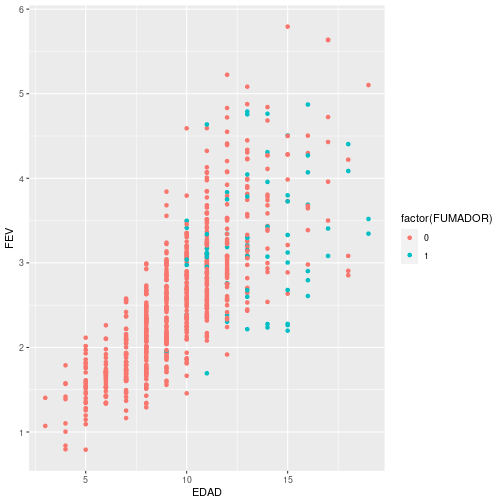
\includegraphics{tablacontingencia_files/figure-beamer/unnamed-chunk-4-1.pdf}

\end{frame}

\begin{frame}[fragile]

\begin{verbatim}
## 
## Frequency table:
##          consume
## curso     No Si
##   Primero 65 40
##   Tercero 56 21
##   Sexto   37 21
\end{verbatim}

\end{frame}

\begin{frame}[fragile]

\begin{verbatim}
##               consuniv$consume
## consuniv$curso    No    Si
##        Primero 69.12 35.88
##        Tercero 50.69 26.31
##        Sexto   38.18 19.82
\end{verbatim}

\end{frame}

\begin{frame}[fragile]

Calculemos el valor del estadístico y su significación:

\begin{verbatim}
## 
##  Pearson's Chi-squared test
## 
## data:  consuniv$curso and consuniv$consume
## X-squared = 2.4548, df = 2, p-value = 0.2931
\end{verbatim}

\end{frame}

\begin{frame}

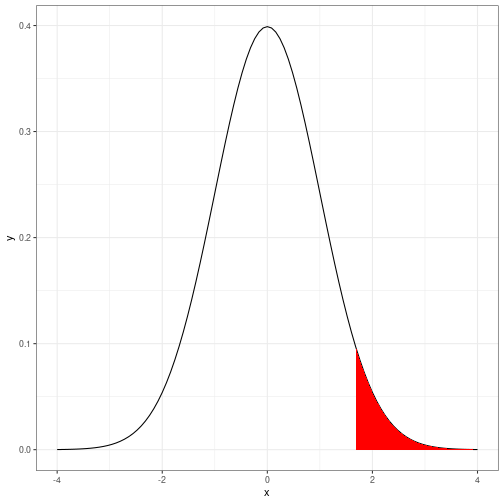
\includegraphics{tablacontingencia_files/figure-beamer/unnamed-chunk-8-1.pdf}

\end{frame}

\begin{frame}

\begin{block}{Condiciones de aplicación de ji-cuadrado}

\begin{itemize}
\tightlist
\item
  Frecuencias esperadas \textgreater{} 5\\
\item
  Si Esperada \textless{} 5, no debe haber más del 25\% celdas\\
\item
  Ninguna Esperada = 0
\end{itemize}

\end{block}

\end{frame}

\end{document}
